%% =====================================================================
\section{Trace-Driven Evaluation}\label{sec:results}
%% =====================================================================
We evaluate CA-DPP on real classifier outputs, replayed over a simulated air-to-ground link. Replaying real outputs matters here: the on-board errors in the traces are correlated in time and only approximately calibrated, so they test the policy under conditions that violate Assumption~\ref{as:inf}.

\subsection{Data}
We build the traces from the hand-labeled part of Sen1Floods11~\cite{bonafilia2020sen1floods11}. It contains 446 Sentinel-2 chips of $512\times512$ pixels at $10$\,m resolution from eleven flood events on several continents, with per-pixel water labels and official train, validation and test splits. No UAV flood dataset with pixel labels of comparable size exists, so this imagery stands in for the UAV view.

To turn a chip into a sequence of frames, a $64\times64$-pixel footprint scans the chip along a serpentine path with a stride of $32$ pixels, one footprint per slot. Consecutive footprints therefore overlap by half, as consecutive frames of a UAV flying at constant speed would. This scan gives the sequence of photos; the position of the UAV, which sets the link, follows the route described below and is generated separately (see Section~\ref{sec:discussion}). A footprint is labeled flooded if at least $10\%$ of its labeled pixels are water, and footprints with less than $80\%$ labeled pixels are skipped. This leaves $46{,}774$, $16{,}612$ and $16{,}811$ slots in the train, validation and test splits. The resulting state sequence is strongly correlated: on the training split, $p_0=0.039$ and $p_1=0.166$, so a dry stretch lasts $26$ slots on average and a flooded stretch $6$ slots.

\subsection{Classifiers}
The on-board model must fit a small processor. We use a logistic regression on the $8\times8$ average-pooled blue, green, red and near-infrared bands, which has $257$ parameters. The ground model can be much larger. We use a gradient-boosted tree ensemble with $300$ trees on $77$ statistics of all $13$ bands and two water indices. Both models are trained on the training split and calibrated by isotonic regression on the validation split.

To study weaker on-board models, we add Gaussian noise of $2$, $4$, $6$ and $8$ times the per-band standard deviation to the input of the on-board model and recalibrate it. On the $174$ validation and test chips ($33{,}423$ slots, $20.5\%$ of them flooded), the five on-board variants are correct on $91.8\%$, $89.4\%$, $86.7\%$, $83.9\%$ and $81.8\%$ of the slots, and the ground model on $97.6\%$. The noise also makes the on-board errors lopsided: the noisiest variant labels $7\%$ of the test slots as flooded, against $21\%$ in truth, so most of its errors are missed floods. Calibration keeps its confidences honest (Fig.~\ref{fig:inference}(a)), so a calibrated controller can still tell when such a model is unsure.

\subsection{Scenario}
Table~\ref{tab:params} lists the scenario parameters. Over one orbit of $200$\,s, the distance to the GS ranges from $0.2$ to $2.8$\,km. The link parameters give a label energy of about $20$\,mJ everywhere and a raw upload that costs $58$ to $420$\,mJ and succeeds with probability $0.99$ to $0.25$, depending on the distance. Blockage has $\rho_{\rm b}=0.02$ and $\rho_{\rm u}=0.1$, so $17\%$ of the slots are blocked, for $10$ slots on average. We consider budgets $\bar E$ from $0.25$ to $10$\,mJ per slot. At the lowest budget the UAV can afford a label in about one slot in $80$, and at the highest it can afford a raw upload in most slots near the GS.

\begin{table}[t]
\caption{Scenario parameters}\label{tab:params}
\centering\footnotesize
\begin{tabular}{@{}ll@{}}
\toprule
Parameter & Value\\
\midrule
Slot length $\tau$; transmission window $\tau_{\max}$ & $0.5$\,s; $0.4$\,s\\
UAV altitude; orbit radius; center to GS & $100$\,m; $1.3$\,km; $1.5$\,km\\
Orbit period & $400$ slots\\
Carrier; bandwidth $W$; transmit power & $2.4$\,GHz; $1$\,MHz; $20$\,dBm\\
Noise figure; environment & $7$\,dB; urban~\cite{alhourani2014lap}\\
Blockage $\rho_{\rm b}$; $\rho_{\rm u}$ & $0.02$; $0.1$\\
Label size $L_1$; frame size $L_2$ & $32$\,B; $50$\,kB\\
Radio power $P_{\rm r}$; overhead $E_{\rm o}$ & $1$\,W; $20$\,mJ\\
Source $p_0$; $p_1$ (training split) & $0.039$; $0.166$\\
Belief support $\Delta_{\max}$ & $300$\\
Energy budget $\bar E$ & $0.25$ to $10$\,mJ/slot\\
\bottomrule
\end{tabular}
\end{table}

\subsection{Baselines and Ablations}
No prior policy addresses our exact problem, so we adapt the four closest designs. All baselines observe the same labels, confidences and link states as CA-DPP. They stay within the budget through a token bucket with an initial credit of $0.5$\,J. When a raw upload does not fit in the bucket, they send the label instead if they can.
\begin{itemize}
\item \emph{AoII threshold}, after~\cite{zakeri2023aoiieh}. The source model there has no classifier, so the UAV treats its label as the observed state. It sends the label once the label has disagreed with the GS for $k\in\{1,2,3,5\}$ consecutive slots. This baseline is the strongest one, because it already ignores agreeing labels.
\item \emph{Pre-identification}, after~\cite{gan2025taoi}. The UAV reports every label and uploads the frames labeled flooded, which the ground model re-identifies.
\item \emph{Age threshold}, after~\cite{pehlivanoglu2026orbit}. Once $A\in\{1,3,10\}$ slots have passed since the last delivery, the UAV uploads the frame if $q_2(g)\ge q^\star$, with $q^\star\in\{0.5,0.9\}$ or never, and sends the label otherwise.
\item \emph{Always offload}, after~\cite{basnayaka2025aomi}. The UAV uploads the frame once $N\in\{1,2,5,10,50\}$ slots have passed since the last delivery and never sends labels.
\end{itemize}
Two ablations isolate parts of CA-DPP. The \emph{confidence-blind} version replaces the confidence $c(t)$ by the precision of the label value on tuning data, i.e., by $\Prob\{X=\lab\mid\lab(t)=\lab\}$. Its belief still uses the class prior, and it still distinguishes ``flooded'' labels from ``dry'' ones, but it treats all frames with the same label alike. The \emph{label-only} version never uploads raw data. Finally, a \emph{genie} that knows $X(t)$ and sends an error-free update whenever the GS is wrong gives a floor for the AoII.

\subsection{Evaluation Protocol}
Chips from the same flood event look alike, so results from a single tuning/test split depend strongly on which chips fall in each set. In preliminary experiments that tuned on the official validation split and tested on the test split, the gains of CA-DPP were much larger than under the cross-validation below, because the chips of the two splits differ systematically. We therefore use $5$-fold cross-validation over the $174$ validation and test chips. For each fold, every parameter is chosen on the other four folds. For CA-DPP and its ablations these are $V$ (four values per budget, between $10^{-3}$ and $10$) and the belief update ($\nu\in\{0.25,0.5\}$ with the class prior, or the symmetric update). For the baselines they are the thresholds listed above. The same four folds give the source statistics, the ground error $\ee_{\rm g}(c)$ in seven confidence bins, and the label precisions of the confidence-blind version. Among the parameter values whose energy stays within $5\%$ of the budget, we keep the one with the lowest AoII.

Each selected policy then runs four times on the held-out fold. Each run visits the chips of the fold four times in random order, with fresh fading and blockage, for about $27{,}000$ slots. This gives $20$ held-out runs per policy and setting. Runs with the same index share all random numbers across policies, so the comparison between two policies is paired. We report means with $95\%$ confidence intervals, paired $95\%$ confidence intervals of the relative change in AoII, paired $t$-tests, and the number of folds in which CA-DPP has the lower mean.

\subsection{AoII Under an Energy Budget}
\begin{table*}[t]
\caption{Trace-driven results at two energy budgets (mean $\pm$ 95\% confidence half-width over 20 held-out runs: 5-fold cross-validation over chips, 4 runs per fold). $\Delta$: change in average AoII obtained by CA-DPP relative to the policy in that row (negative means CA-DPP is lower), with paired 95\% confidence interval, paired $t$-test $p$-value, and the number of folds (out of 5) in which CA-DPP has the lower mean.}
\label{tab:results}
\centering\footnotesize\setlength{\tabcolsep}{3.2pt}
\begin{tabular}{@{}lcccccccc@{}}
\toprule
 & \multicolumn{4}{c}{$\bar E=0.25$\,mJ/slot} & \multicolumn{4}{c}{$\bar E=2$\,mJ/slot}\\
\cmidrule(lr){2-5}\cmidrule(l){6-9}
Policy & AoII & $\Delta$ (\%) & $p$ & folds & AoII & $\Delta$ (\%) & $p$ & folds\\
\midrule
CA-DPP (proposed) & $0.645\pm0.165$ & -- & -- & -- & $0.390\pm0.085$ & -- & -- & -- \\
AoII threshold~\cite{zakeri2023aoiieh} & $0.925\pm0.258$ & $-22.3\pm11.6$ & $0.002$ & 4/5 & $0.352\pm0.060$ & $+9.5\pm13.2$ & $0.171$ & 3/5 \\
Pre-identification~\cite{gan2025taoi} & $2.556\pm0.284$ & $-74.8\pm6.2$ & $<\!10^{-3}$ & 5/5 & $0.796\pm0.129$ & $-52.0\pm5.2$ & $<\!10^{-3}$ & 5/5 \\
Age threshold~\cite{pehlivanoglu2026orbit} & $2.538\pm0.381$ & $-74.8\pm4.2$ & $<\!10^{-3}$ & 5/5 & $0.784\pm0.114$ & $-51.8\pm5.1$ & $<\!10^{-3}$ & 5/5 \\
Always offload~\cite{basnayaka2025aomi} & $12.451\pm1.288$ & $-94.5\pm1.5$ & $<\!10^{-3}$ & 5/5 & $8.444\pm0.869$ & $-95.2\pm1.1$ & $<\!10^{-3}$ & 5/5 \\
\midrule
CA-DPP, confidence-blind & $0.739\pm0.165$ & $-13.3\pm5.2$ & $0.001$ & 4/5 & $0.345\pm0.056$ & $+10.3\pm9.9$ & $0.051$ & 2/5 \\
CA-DPP, label only & $0.686\pm0.204$ & $+6.7\pm13.8$ & $0.487$ & 1/5 & $0.428\pm0.101$ & $-7.1\pm3.0$ & $0.001$ & 4/5 \\
\midrule
Genie (knows $X$) & \multicolumn{8}{l}{AoII $0.171\pm0.011$, $\Prob$(GS wrong) $0.070$, energy $0.96$\,mJ/slot when unconstrained} \\
\bottomrule
\end{tabular}
\end{table*}


\begin{figure*}[t]
\centering
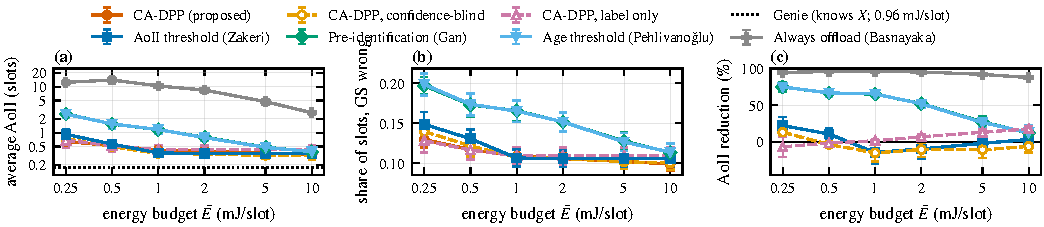
\includegraphics[width=\textwidth]{figures/fig_budget.pdf}
\caption{Energy budget sweep, $20$ held-out runs per point, with $95\%$ confidence intervals. (a) Average AoII. (b) Fraction of slots in which the GS is wrong. (c) AoII reduction by CA-DPP relative to each policy (paired intervals); negative values favor the other policy. Baselines are adapted from Zakeri et al.~\cite{zakeri2023aoiieh}, Gan et al.~\cite{gan2025taoi}, Pehlivano\u{g}lu et al.~\cite{pehlivanoglu2026orbit} and Basnayaka et al.~\cite{basnayaka2025aomi}.}
\label{fig:budget}
\end{figure*}

Fig.~\ref{fig:budget} and Table~\ref{tab:results} summarize the results. Against the pre-identification and age-threshold policies, CA-DPP lowers the AoII by $75\%$ at $0.25$\,mJ/slot, $52\%$ at $2$\,mJ/slot and $12\%$ at $10$\,mJ/slot, in every fold up to $5$\,mJ/slot ($p<10^{-5}$). The pre-identification policy spends most of its energy on labels that confirm what the GS already believes, which Proposition~\ref{prop:confirm} shows to be worthless. The age-threshold policy reacts to the time since the last delivery, which says little about whether the GS is wrong: an old status of a dry area that is still dry needs no update. Offloading every update is an order of magnitude worse at every budget, because a raw frame costs as much as $3$ to $21$ labels and fails often far from the GS.

Against the AoII-threshold policy, the outcome depends on the budget. At $0.25$\,mJ/slot, CA-DPP lowers the AoII by $22\%\pm12\%$ ($p=0.002$, four folds of five), and the $99$th percentile of the AoII drops from $19.2$ to $12.3$ slots. Here the UAV can send few labels, and the confidence decides which disagreements deserve them. At $0.5$\,mJ/slot the reduction is $11\%\pm7\%$ and not significant ($p=0.10$). From $1$\,mJ/slot on, the threshold policy with $k=1$ reports every disagreement for about $0.84$\,mJ/slot and matches CA-DPP; the differences range from $-3\%$ to $+14\%$ with $p\ge0.09$. When labels are this cheap, a wrong label is corrected by the next frame within a slot or two, which the one-step gain of Lemma~\ref{lem:onestep} ignores. We tested a discounted look-ahead over several slots of silence in place of the one-step gain, and it did not help.

\begin{figure}[t]
\centering
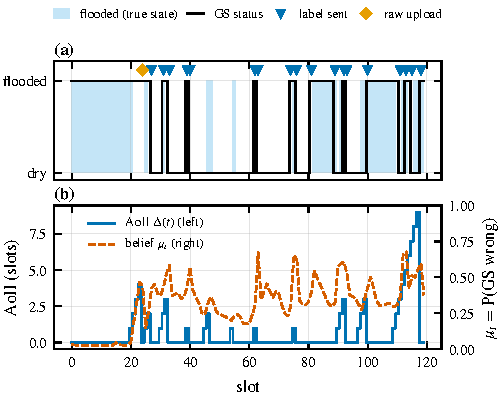
\includegraphics[width=\columnwidth]{figures/fig_path.pdf}
\caption{A sample path of CA-DPP at $\bar E=0.5$\,mJ/slot ($V=0.01$, $\nu=0.25$). (a) True state (shaded when flooded), GS status, and the slots in which the UAV sends a label (triangles) or uploads the frame (diamond). (b) AoII of the GS status (left axis) and the belief $\mu_t$ that the GS is wrong (right axis).}
\label{fig:path}
\end{figure}

Fig.~\ref{fig:path} shows CA-DPP over $120$ slots. The belief $\mu_t$ rises with each disagreeing frame; once it is high enough, the UAV sends a label and the AoII returns to zero. Over flooded stretches with patchy water, the classifier and the scene disagree often, and the UAV sends several labels in quick succession. A short AoII spike at the end of the window shows the cost of waiting: the belief rose more slowly than the true error, because the tempered update discounts the first disagreeing frames.

\subsection{Where the Gains Come From}
The ablations separate the contribution of the per-frame confidence from that of the raw uploads. At $0.25$\,mJ/slot the per-frame confidence matters: the confidence-blind version has a $15\%$ higher AoII ($p=0.001$). From $1$\,mJ/slot on, however, the confidence-blind version is $6\%$ to $15\%$ better than CA-DPP, and the difference is significant only at $1$\,mJ/slot ($p=0.02$). With this classifier, once energy is not scarce, the precision of each label value gives the belief most of what it needs. A plausible reason is the correlation of the on-board errors. A confident wrong label is often followed by another confident wrong label, and the per-frame update, even tempered, then raises the belief faster than it should. The per-label precision averages over such runs and is more robust to them.

Raw uploads pay off at larger budgets. Without them, the AoII stays at $0.43$ from $1$\,mJ/slot on, since the label-only version runs out of useful labels to send and spends only $0.65$\,mJ/slot. CA-DPP spends the rest of the budget on uploads and reaches $0.39$ at $2$\,mJ/slot and $0.34$ at $10$\,mJ/slot ($p\le0.001$). The genie reaches an AoII of $0.171$ with $0.96$\,mJ/slot. Most of the gap to it comes from not observing $X(t)$, which no policy can avoid.

\subsection{Weak Classifiers, Blockage and Payload}
\begin{figure*}[t]
\centering
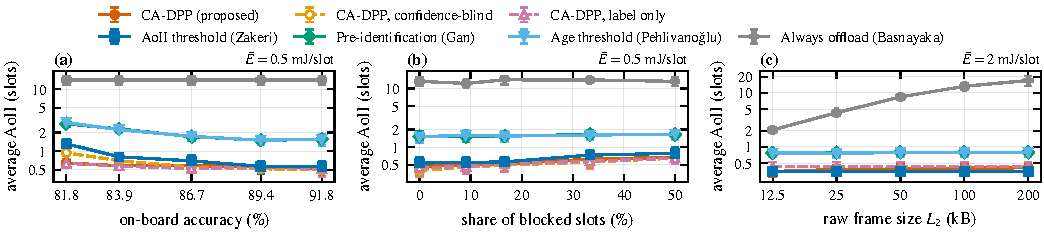
\includegraphics[width=\textwidth]{figures/fig_sensitivity.pdf}
\caption{Sensitivity, $20$ held-out runs per point. (a) On-board accuracy and (b) share of blocked slots, $\rho_{\rm b}/(\rho_{\rm b}+\rho_{\rm u})$, at $\bar E=0.5$\,mJ/slot. (c) Raw frame size at $\bar E=2$\,mJ/slot.}
\label{fig:sens}
\end{figure*}

Fig.~\ref{fig:sens}(a) lowers the on-board accuracy at $0.5$\,mJ/slot. The AoII of CA-DPP grows only from $0.53$ to $0.64$ as the accuracy drops from $91.8\%$ to $81.8\%$. Over the same range, the AoII of the threshold policy grows from $0.56$ to $1.31$, and that of the confidence-blind version from $0.50$ to $0.94$. At $86.7\%$ accuracy, CA-DPP is $12\%$ better than the threshold policy ($p=0.006$). With the two noisiest models, it is $27\%$ and $49\%$ better than the threshold policy ($p<10^{-5}$) and $14\%$ and $28\%$ better than the confidence-blind version ($p\le0.003$), in all five folds. With the two most accurate models the three policies are within the run-to-run spread. The noisiest model rarely says ``flooded'', so over a flooded area it mostly agrees with the wrong ``dry'' status of the GS. The threshold policy, which reacts only to disagreements, spends only $0.32$ of $0.5$\,mJ/slot. CA-DPP spends the full budget: a low-confidence ``dry'' frame barely lowers its belief that the GS is wrong, while a rare confident ``flooded'' frame raises it strongly, since flooded footprints are rare. The confidence-blind belief knows that ``dry'' labels are less reliable on average, but not which ones. Per-frame confidence therefore pays off when the classifier is weak and its errors are lopsided, as is likely for a small model on a low-cost device.

As the share of blocked slots grows from $0$ to $50\%$ (Fig.~\ref{fig:sens}(b)), all policies lose ground and their order is unchanged. CA-DPP stays $9\%$ to $15\%$ below the threshold policy ($0.009\le p\le0.1$). The confidence-blind and label-only versions are $1.5\%$ to $11\%$ below CA-DPP at this budget, so at $0.5$\,mJ/slot raw uploads cost slightly more than they return. Fig.~\ref{fig:sens}(c) varies the size of the raw frame at $2$\,mJ/slot. With $12.5$\,kB frames, CA-DPP is $15\%$ better than the label-only version and matches the threshold policy. With $200$\,kB frames the advantage over label-only shrinks to $3.5\%$, because uploads become more expensive and less reliable, and the policy uploads less often without any retuning.

\subsection{The Weight $V$ and the Role of Mobility}
\begin{figure}[t]
\centering
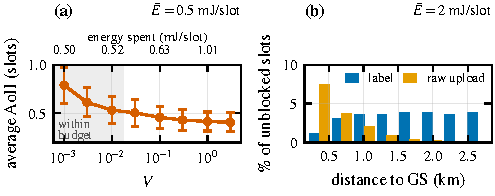
\includegraphics[width=\columnwidth]{figures/fig_V_mix.pdf}
\caption{(a) AoII of CA-DPP versus $V$ at $\bar E=0.5$\,mJ/slot; the top axis gives the energy spent, and the shaded values of $V$ stay within $4\%$ of the budget. (b) Share of unblocked slots with a label or a raw upload versus the distance to the GS, at $\bar E=2$\,mJ/slot.}
\label{fig:Vmix}
\end{figure}

Fig.~\ref{fig:Vmix}(a) shows the trade-off governed by $V$ at $0.5$\,mJ/slot. Raising $V$ from $10^{-3}$ to $3$ lowers the AoII from $0.79$ to $0.41$. A larger $V$, however, lets the energy debt grow larger before it raises the price, and over a run of about $27{,}000$ slots the energy spent rises from $0.50$ to $1.51$\,mJ/slot. Values of $V$ up to $10^{-2}$ stay within $4\%$ of the budget. This is the finite-horizon face of Theorem~\ref{thm:budget}: the budget is met in the long run for every $V$, but the transient excess grows with $V$, so $V$ must be matched to the mission length.

Fig.~\ref{fig:Vmix}(b) shows how CA-DPP exploits the trajectory at $2$\,mJ/slot. Within $850$\,m of the GS, where uploads are cheap and reliable, it uploads the frame in $5.9\%$ of the unblocked slots and sends labels in $2.0\%$. Beyond $2.15$\,km it uploads in only $0.1\%$ and sends labels in $3.8\%$. The UAV thus asks the ground when asking is cheap and relies on its own labels when it is not, with no rule that refers to the distance explicitly. The distance enters only through $q_a(g)$ and $E_a(g)$ in~\eqref{eq:rule}.
